\documentclass[a4paper,11pt]{article}
\usepackage[margin=1.25in, top=1.5in,bottom=1.5in]{geometry}
\usepackage{amsmath}
\usepackage{gensymb}
\usepackage{graphicx}
\usepackage{mathtools}
\usepackage{booktabs}
\usepackage{multirow}
\usepackage{mathtools}
\usepackage{caption}
\usepackage{parskip}
\usepackage{tikz}
\usepackage{hyperref}
\renewcommand\rmdefault{ptm} % use Times
\let\boldtheta\theta % make theta into vector
\renewcommand{\theta}{\boldsymbol{\boldtheta}} % make theta into vector
\renewcommand{\d}{\: \mathrm{d}} % fix d in integrals
\usepackage{scrextend} % for lists

\title{\vspace*{-1.75em}\textbf{Project Proposal}\\ \vspace{0.25em} \Large Investigating improvements to approximate Bayesian inference in Variational Continual Learning}

\author{M. E. Tong, supervised by S. Farquhar and Y. Gal}

\date{}

\begin{document}

\maketitle

%Background: the theory or application areas;
%General open questions;
%Selection of particular question for study;
%Proposed method;
%Draft Timetable;
%Signature of Project Supervisor.

For real-world problems, it is vital that intelligent agents have the capacity to learn and remember a variety of tasks \cite{overcoming}. Continual learning refers to online multi-task learning where tasks are learned sequentially, with datasets discarded after training. It is of particular importance for applications for which retaining old datasets is unethical, undesireable, illegal or imprudent \cite{unifying, robust}.

The major problem in the field is that of catastrophic forgetting. New learning often causes neural networks to rapidly forget old learning \cite{catastrophic}. The challenge is to balance learning new tasks whilst remembering previous ones. Though promising results have been published in the field of continual learning, clear shortcomings have been identified in many of the current approaches and evaluations \cite{robust}. % Mention that some approaches require retaining previous datasets - cheating!

We suggest that further investigation into the Variational Continual Learning (VCL) approach \cite{vcl} is warranted.

VCL demonstrates a Bayesian approach to continual learning, where the posterior for the previous tasks is used as the prior when training on the new task dataset. This allows the previous tasks to strongly influence prediction, whilst allowing the parameters to adapt to the new task. 
\begin{equation}\label{eq:1}
\begin{split}
\underbrace{p(\theta | \mathcal{D}_{1:t})}_{\mathclap{\text{new posterior}}} \propto \underbrace{p(\theta | \mathcal{D}_{1:t-1})}_{\substack{\text{previous posterior}\\ (\text{new prior})}} \underbrace{p(\mathcal{D}_t | \theta)}_{\text{likelihood}}
\end{split}
\end{equation}

However, the true posterior $p(\theta | \mathcal{D}_{1:t})$ is computationally intractable, so we must approximate it. We suggest that improvements to this approximation may be key to performance. 

The posterior approximation in VCL is performed using Kullback-Leibler (KL) minimisation, a variational method, over a model family of possible posteriors $\mathcal{Q}$, to yield a tractable normalised approximation $q_t(\theta)$. We define $q_0(\theta)$ to be the prior, $p(\theta)$.
\vspace{-0.5em}
\begin{equation}\label{eq:3}
\begin{split}
\underbrace{q_t(\theta)}_{\mathclap{\substack{\text{new posterior}\\ \text{approximation}}}} &=\underset{q\in\mathcal{Q}}{\mathrm{arg}\mathrm{min}} \: \mathrm{KL}\bigg(q(\theta)\:||\:\frac{1}{Z_t}\underbrace{q_{t-1}(\theta)}_{\mathclap{\substack{\text{previous posterior} \\ \text{approximation}}}}p(\mathcal{D}_t|\theta) \bigg)\\
& \approx \underbrace{p(\theta | \mathcal{D}_{1:t})}_{\mathclap{\substack{\text{new true posterior}}}}
\end{split}
\end{equation}

Here, $\theta$ are the parameters, $\mathcal{D}_i$ is the $i$\textsuperscript{th} dataset, $q_i(\theta)$ is the posterior approximation following the $i$\textsuperscript{th} dataset, $Z_t$ is the intractable normalisation constant which is irrelevant for minimisation.

Crucially, this is exact Bayesian inference, i.e.\ $q_t(\theta)=p(\theta | \mathcal{D}_{1:t}) \: \forall t$, if two criteria are met at every step:

\begin{enumerate}
\item The true posterior is a member of the model family $\mathcal{Q}$.
\item The optimisation achieves the minimum KL divergence.
% Optimisation is a big problem, as we aren't sure that we find the minimum
% We make a big assumption that we are actually getting a minimum KL divergence
\end{enumerate}

Since the posterior approximation occurs after every task is learned, improving this approximation is important to prevent error propagation across different tasks.

We suggest that investigation into an improvement to the first criterion is most promising, as we suspect that it is likely that the model family used in VCL is not sufficient to approximate the posterior well. The primary aim of the project is therefore to see if using a more adaptable model family results in better performance:
% So we're pretty confident it doesn't lie in this model family
% Relaxation

\begin{enumerate}
\item \textbf{Using full covariance Gaussian distributions for the model family $\mathcal{Q}$.}

VCL uses a Gaussian mean-field approximate posterior, with diagonal covariance: %sigma^2_{t,d}
\[q_t(\theta) = \prod^D_{d=1} \mathcal{N}(\boldtheta_{t,d}; \mu_{t,d}, \sigma^2_{t,d})\]

% correlation elements, non-diagonal elements
We expect that a full covariance Gaussian distribution will be able to approximate the posterior more accurately, as the covariance matrix has off-diagonal correlation elements. `More flexible distributions \ldots\ simply give better approximations to the true posterior' \cite{ensemblelearning}. The minimum KL fit obtained with the full covariance model family should therefore be better than that obtained with the diagonal covariance model family.
\begin{center}
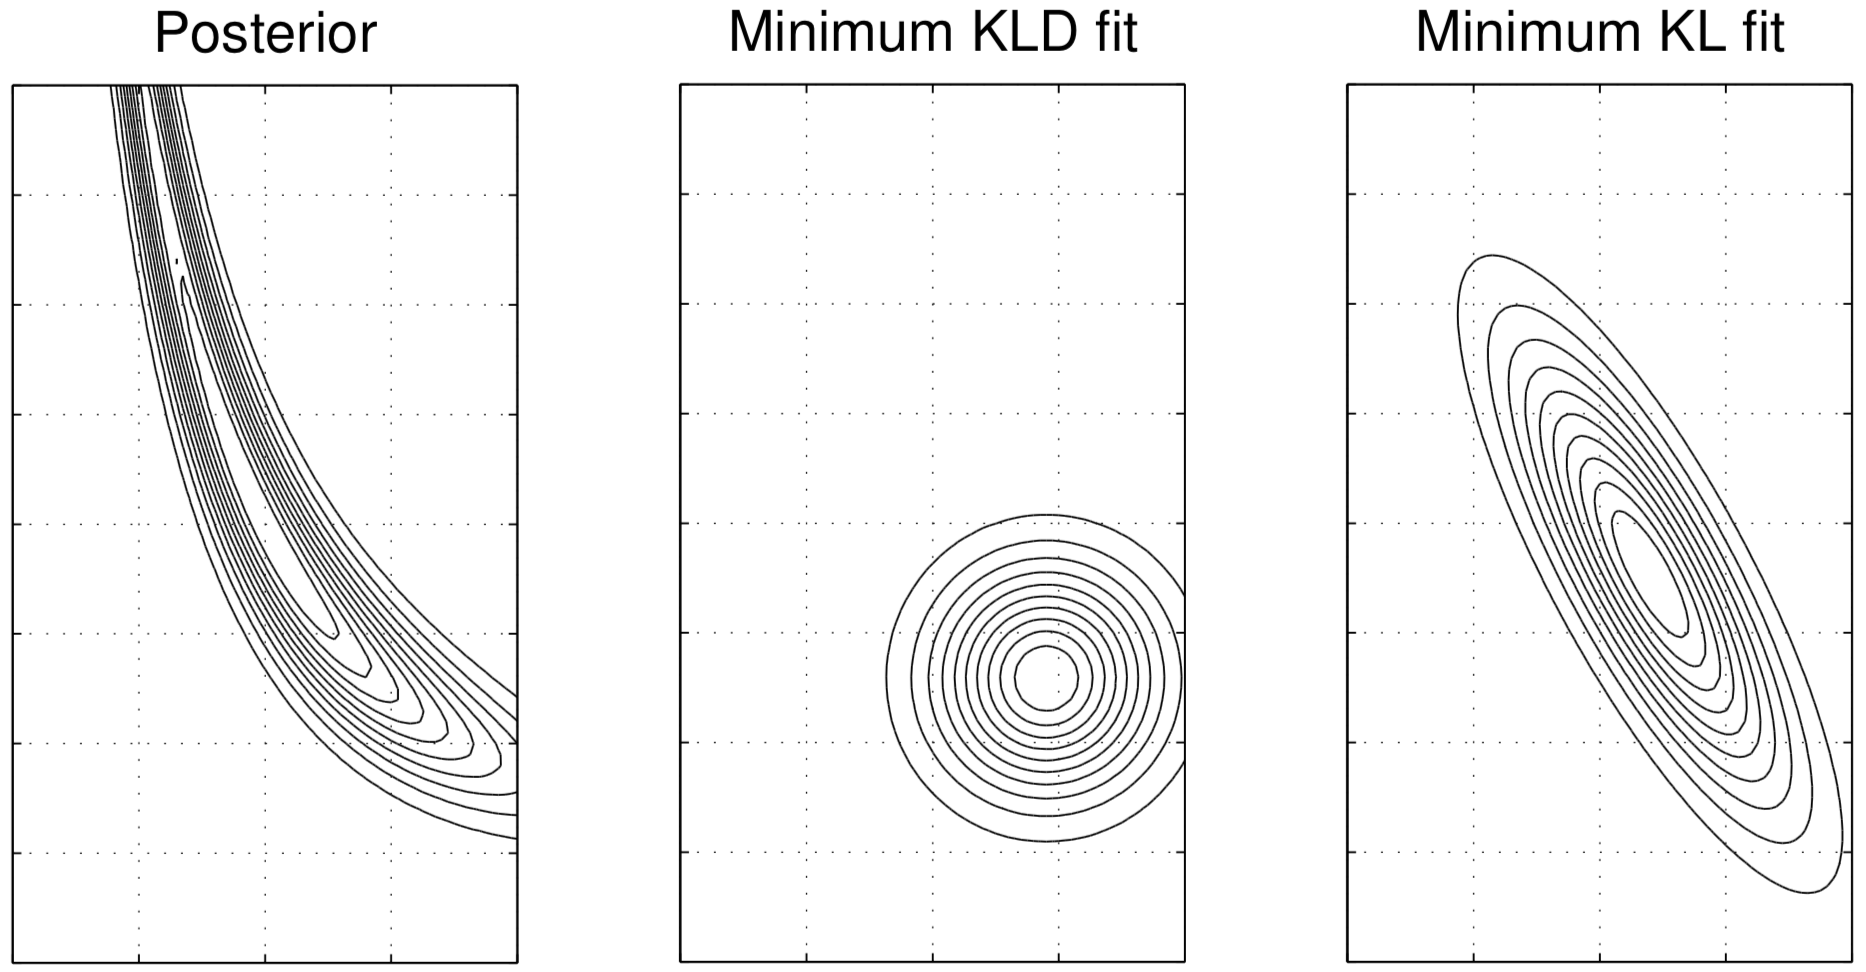
\includegraphics[width=0.6\textwidth]{approximations}
 \captionof{figure}{Comparison of posterior distribution approximations on a synthetic example with two parameters. A diagonal covariance Gaussian distribution (KLD) results in KL\textsubscript{res} = 4.6, whereas a full covariance Gaussian distribution (KL) results in KL\textsubscript{res} = 3.9. \cite{ensemblelearning}}.
 \label{figure:family}
\end{center}

\newpage

Approximate Bayesian inference is typically done with either variational or Markov Chain Monte Carlo (MCMC) inference. We also suggest investigation into using a MCMC approach instead of variational approach such as KL minimisation. The secondary aim of the project is therefore to see if using MCMC results in better performance:

\item \textbf{Using a Markov Chain Monte Carlo method for posterior approximation.}

We expect that Hamiltonian Monte Carlo (HMC) is a good MCMC method to use for approximate inference. HMC is a principled Hamiltonian dynamics-based MCMC method which has been applied successfully to Bayesian neural networks \cite{bayesianlearning}. It systematically and coherently traverses the state space, avoiding the slow exploration typical of random walk proposals \cite{hmc}. This is particularly useful in high-dimensional spaces, where we must use information about the space geometry for an efficient exploration. Gradient-based algorithms such as HMC tend to be more robust and geometrically ergodic over a larger class of target distributions than non-gradient based algorithms, yielding `stronger guarantees on the validity of the resulting estimators' \cite{conceptual}.
% second-gradient - calculating Hamiltonian is really expensive for high dimensional spaces
% HMC sets cap on size of neural network we can use
\end{enumerate}


\subsection*{Timeline}

\begin{tabular}{l|l}
\hline
March 	& Write project proposal; review literature\\
April	& Use non-continual BNN to compare diagonal and full model families\\
May		& Continue with comparison; begin to implement continual learning comparison\\
June 	& Continue continual learning comparison implementation\\
July	& Begin with Markov Chain Monte Carlo implementation\\
August	& Continue with MCMC implementation\\
September 2 & Hand-in date\\
\hline
\end{tabular}

\subsection*{Project supervisors' signatures}

\begin{labeling}{projectsupervisors}
\vspace*{2.25em}
\item[S. Farquhar] \rule{5cm}{1pt}
\vspace*{2.5em}
\item[Y. Gal] \rule{5cm}{1pt}
\end{labeling}


 

\newpage
\begin{thebibliography}{8}

\bibitem[Farquhar \& Gal, 2019]{unifying} S. Farquhar, Y. Gal, 2019. \textit{A Unifying Bayesian View of Continual Learning}. arXiv:1902.06494v1

\bibitem[Farquhar \& Gal, 2018]{robust} S. Farquhar, Y. Gal, 2018. \textit{Towards Robust Evaluations of Continual Learning}. arXiv:1805.09733v2

\bibitem[Nguyen et al., 2017]{vcl} C. V. Nguyen, Y. Li, T. D. Bui, R. E. Turner, 2017. \textit{Variational Continual Learning}. arXiv:1710.10628v3
 
\bibitem[Betancourt, 2017]{conceptual} M. Betancourt, 2017. \textit{A Conceptual Introduction to Hamiltonian Monte Carlo}. arXiv:1701.02434v2

\bibitem[Kirkpatrick et al., 2016]{overcoming} J. Kirkpatrick, R. Pascanua, N. Rabinowitza, J. Venessa, G. Desjardinsa, A. A. Rusua, K. Milana, J. Quana, T. Ramalhoa, A. Grabska-Barwinskaa, D. Hassabisa, C. Clopathb, D. Kumarana, and R. Hadsella, 2017. \textit{Overcoming catastrophic forgetting in neural networks}. arXiv:1612.00796v2

\bibitem[Neal, 2012]{hmc} R. M. Neal, 2012. \textit{MCMC using Hamiltonian dynamics}. arXiv:1206.1901v1

%\bibitem[Liu \& Chen, 1998] J. S. Liu, R. Chen, 1998. \textit{Sequential Monte Carlo Methods for Dynamic Systems}. Journal of the American Statistical Association, Vol. 93, No. 443, pp. 1032-1044.

\bibitem[Barber \& Bishop, 1998]{ensemblelearning} D. Barber, C. M. Bishop, 1998. \textit{Ensemble Learning in Bayesian Neural Networks}. Neural Networks and Machine Learning, Springer, 215-237. \url{https://www.microsoft.com/en-us/research/wp-content/uploads/2016/02/bishop-ensemble-nato-98.pdf}

\bibitem[Neal, 1995]{bayesianlearning} R. M. Neal, 1995. \textit{Bayesian Learning for Neural Networks}. \url{http://citeseerx.ist.psu.edu/viewdoc/download?doi=10.1.1.446.9306&rep=rep1&type=pdf}

%\bibitem[Ratcliff, 1990]{connectionist} R. Ratcliff, 1990. \textit{Connectionist Models of Recognition Memory: Constraints Imposed by Learning and Forgetting Functions}. Psychological Review, Vol.97, No. 2, 285-308.

\bibitem[McCloskey \& Cohen, 1989]{catastrophic} M. McCloskey, N. J. Cohen, 1989. \textit{Catastrophic Interference in Connectionist Networks: The Sequential Learning Problem}. Psychology of Learning and Motivation, Volume 24, 1989, Pages 109-165.

\end{thebibliography}



\end{document}
